\section{Fisher's linear discriminant} 

\begin{frame}
    \frametitle{Introduction to Fisher's linear discriminant}

    Consider first the case of 
    two classes, and suppose we take the
    $D-$dimensional input vecto $x$ and project it down to one 
    dimension using 
    \begin{equation}\label{eq:05:projection}
        y = w^T x. 
    \end{equation}

    Place a threshold on $y$ and classify
    $y \geq -w_0$ as class $C_1$ otherwise class $C_2$. 

    \textbf{We can select a projection that maximizes the class separation}
\end{frame}

\begin{frame}
    \frametitle{Math formulation: first idea}
    The mean vectors of the two classes are given by

    \begin{equation}
        m_i = 
        \frac{1}{N_i} 
        \sum_{n \in C_i}
    \end{equation}
    where $i \in \{1,2\}$ and there are $N_i$ points of class $C_i$.
    
    The simplest measure of the separation of the classes,
    when projected onto $w$, is the 
    separation of the projected class mean.
    This suggests that we might choose $w$ so as to maximize 
    \begin{equation}
        c_2 - c_2 = w^T (m_2 - m_1)
    \end{equation}
    where 
    \begin{equation}\label{eq:05:proyected_mean}
        c_i = w^T m_i
    \end{equation}
    is the mean of the projected data form class $C_i$. 
\end{frame}

\begin{frame}
    \frametitle{Problem of this approach}
    This expression can be made arbitrarily large simply by increasing the magnitude of $w$. 
    Solution: constrain $w$ to have a unit length so that 

    \begin{equation}
        \sum_i w^2_i = 1.
    \end{equation}
    Use a Lagrange multiplier to perform the constrained maximization,
    we then find that 
    \begin{equation}
        w \propto (m_2 - m_1).
    \end{equation}
\end{frame}

\begin{frame}
    \frametitle{Problems: Overlap when projected}
\begin{figure}[t]
    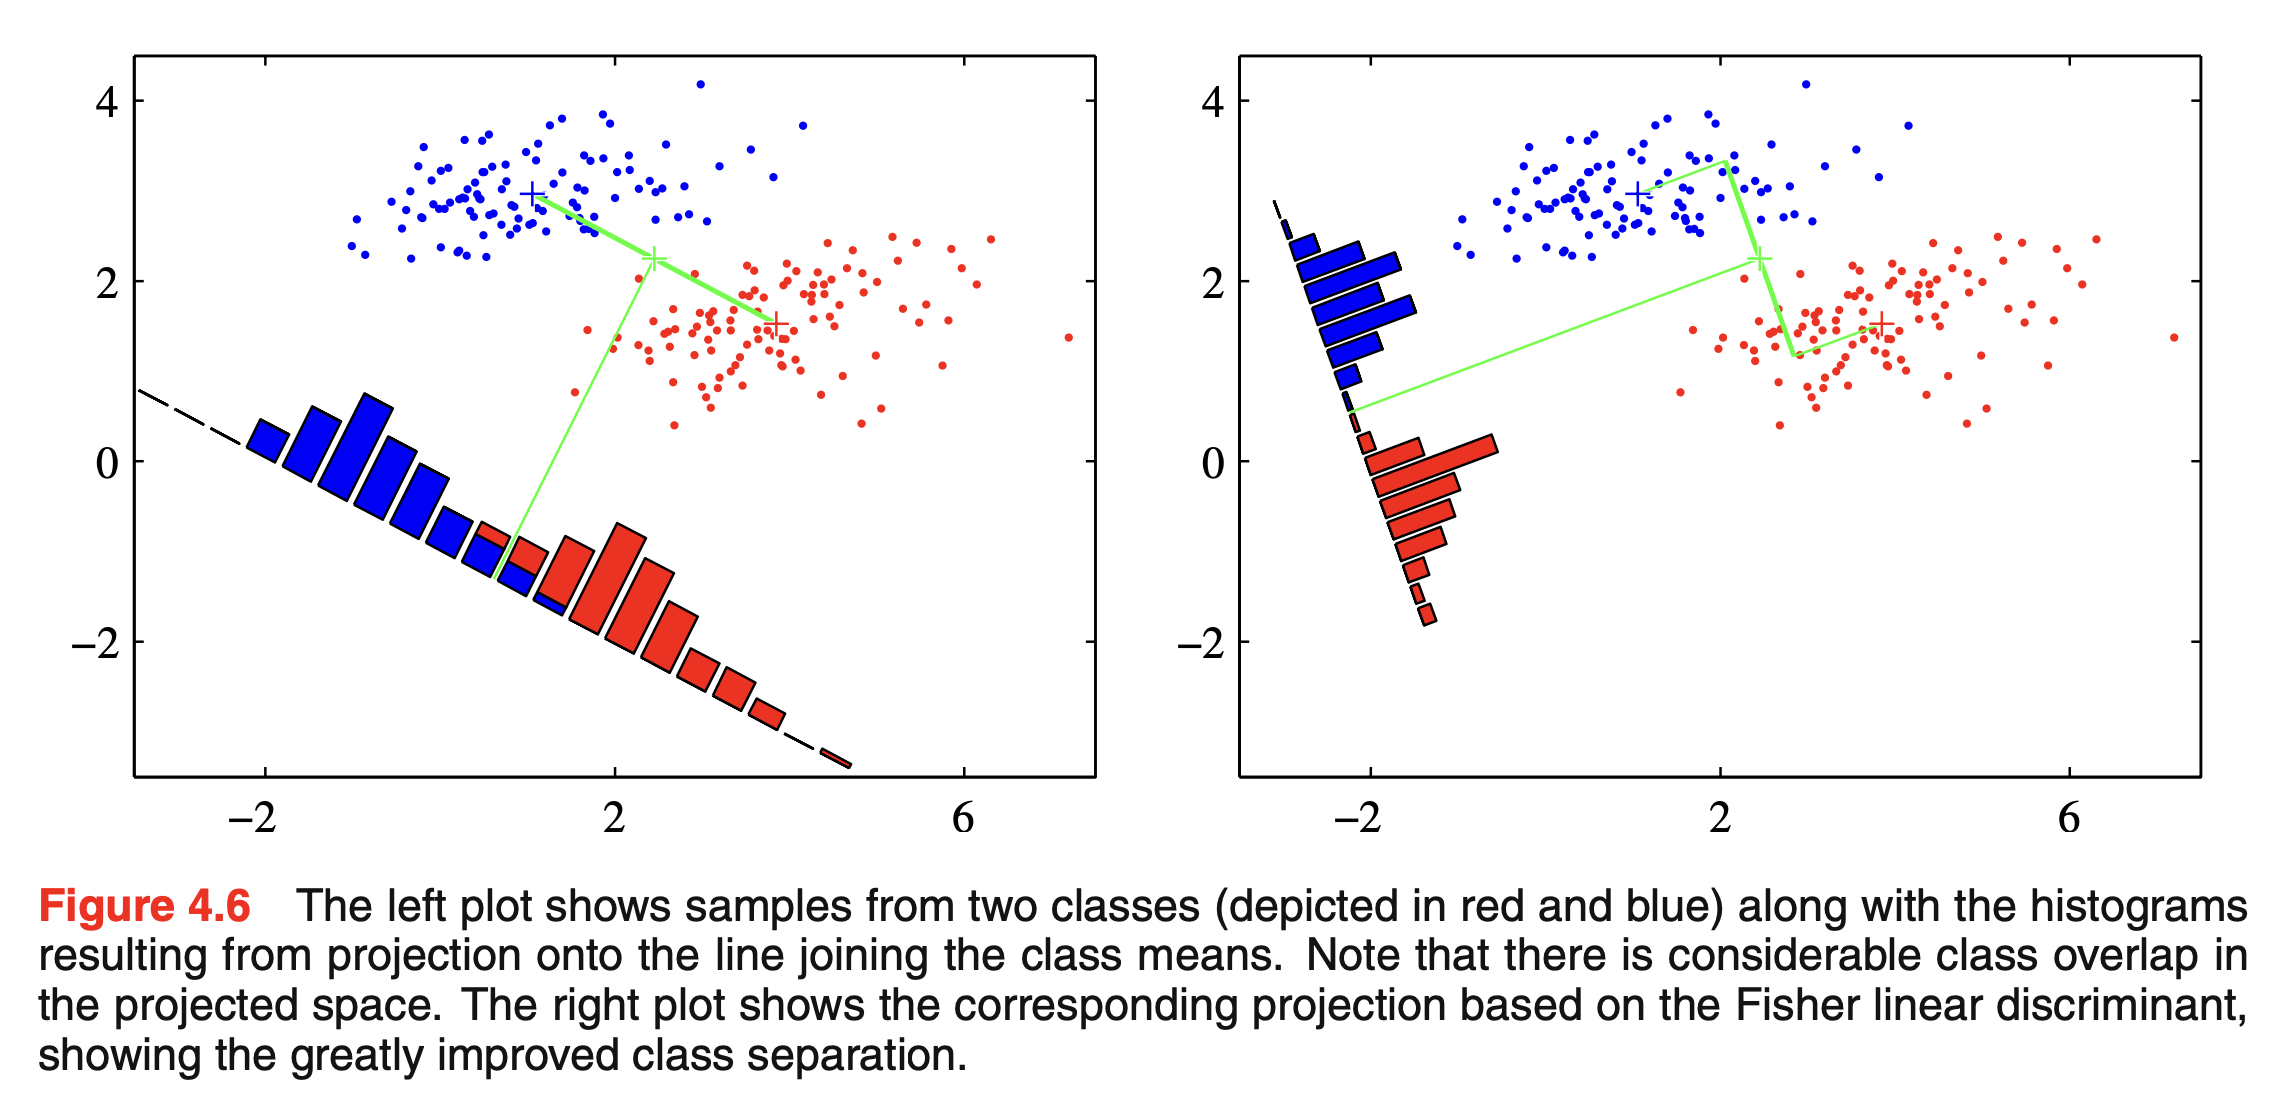
\includegraphics[width=0.95\textwidth]{
        04_Classification/projection_overlap.png
    }
    \centering
\end{figure}

\end{frame}

\begin{frame}
    \frametitle{Fisher's solution}

    Maximize a function a function that will give a large separation between the projected
    class means while also giving a small variance within each class, \textbf{thereby} minimizing the class overlap. 

    the within-class variance of the transformed data
    from class $C_k$ is therefore given by
    \begin{equation}\label{eq:05:variance}
        s_k^2
        = 
        \sum_{n \in C_k}
        \left(
            y_n - c_k
        \right)^2
    \end{equation}
    where $y_n = w^T x_n$.

    We can define the total within-class variance for the whole data set to be simply $s_1^2 + s_2^2$. 
\end{frame}

\begin{frame}
    \frametitle{Fisher criterion definition }

    The Fisher criterion is defined to be the ration 
    of the between-class class variance to the 
    within class variance and is given by 

    \begin{equation}
        J(w)
        = 
        \frac{
            (m_2 - m_1)^2
        }{
            s_1^2 + s_2^2
        }.
    \end{equation}
    We can make the dependence on $w$ 
    explicit by using
    \ref{eq:05:projection}
    \ref{eq:05:proyected_mean}
    \ref{eq:05:variance}
    to rewrite the Fisher criterion in the form
\end{frame}

\begin{frame}
    \frametitle{Fisher explicit form}

    
    \begin{equation}\label{eq:05:explicit}
        J(w)
        = 
        \frac{w^T S_B w}{w^T S_W s}
    \end{equation}
    where $S_B$ is the \ti{between class} covariance matrix and is given by 

    \begin{equation}\label{05:within-class-covariance}
        S_B = 
        (m_2 - m_1)
        (m_2 - m_1)^T
    \end{equation}
    and $S_W$ is the total \textit{within class} covariance matrix, given by
    \begin{equation}
        S_W
        = 
        \sum_{k \in \{1,2\}}
        \sum_{n \in C_i}
            (x_n - m_k)
            (x_n - m_k)^T.
    \end{equation}
\end{frame}


\begin{frame}
    \frametitle{Maximizing}

    Differentiating \ref{eq:05:explicit} with respect to 
    $w$, we find that $J(w)$ is maximized when 
    \begin{equation}\label{eq:05:maximized_J_equation}
        (w^T S_B w)S_W w 
        = 
        (W^T S_W w) S_B w.
    \end{equation}

    Some consideration: 
    \begin{itemize}
        \item From \ref{05:within-class-covariance} we see that $S_B w$ is always in the direction of $(m_2 -m_1)$.
        \item We do not care about the magnitude of $w$, only its direction, and so we can drop the escalar factors $(w^T S_B w)$ and $(w^T S_W w)$. 
    \end{itemize}

    Multiplying both side of \ref{eq:05:maximized_J_equation} by $S^{-1}_W$ we obtain the \textbf{Fisher's linear discriminant}

    \begin{equation}
        w 
        \propto
        S^{-1}_W (m_2 - m_1).
    \end{equation}
    Note that if the within class covariance is isotropic  (proportional to unit matrix), we find that $S_W$ is proportional to the difference of the class mean. 
\end{frame}

\begin{frame}
    \frametitle{Some observation }

    It is not a discriminant but rather 
    a specific choice of direction 
    for projection to one dimension. 
    
    In order to construct a discriminant we can 
    choose a threshold $y_0$ so that we classify a new point as belonging to 
    $C_1$ if $y(x) \geq y_0$. 
\end{frame}

\subsection{Relation between Fisher discriminant and least squares}

\begin{frame}
    \frametitle{Fisher criterion can be obtained as a special case of least squares}

    We shall take the targets for class $C_1$ to be $\frac{N}{N_1}$
    and for class $-\frac{N}{N_2}$. 

    The sum if squares error function can be written 

    \begin{equation}
        E = \frac{1}{2}
        \sum_{n = 1}^N
        (w^T x_n + w_0 - t_n)^2.
    \end{equation}

    Derivatives of $E$ with respect to $w_0$ and $w$ to zero

\end{frame}

\begin{frame}
    \frametitle{erivatives of $E$ with respect to $w_0$ and $w$ to zero}
    \begin{equation}\label{eq:05:w0_derivative}
        \sum_{n = 1}^N (w^T x_n + w_0 - t_n) = 0,
    \end{equation}

    \begin{equation}
        \sum_{n = 1}^N (w^T x_n + w_0 - t_n)x_n = 0.
    \end{equation}
\end{frame}

\begin{frame}
    \frametitle{Working with \ref{eq:05:w0_derivative}}

    Since 
    \begin{equation} \label{eq:05:sum_tn}
        \sum_{n = 1}^N t_n 
        = 
        N_1 \frac{N}{N_1} 
        - 
        N_2 \frac{N}{N_2}
        = 0
    \end{equation}
    and 
    \begin{equation} \label{eq:05:sum_xn}
        \sum_{n = 1}^N x_n 
        = N m
        = N_1 m_1 + N_2 m_2.
    \end{equation}

   Substituting  \ref{eq:05:sum_xn} and   \ref{eq:05:sum_tn} in \ref{eq:05:w0_derivative}
   we obtain an expression for the bias in form 
   \begin{equation}
    w_0 = -w^T m.
   \end{equation}
    

\end{frame}



